Wie schon erwähnt stellt die praktische Umsetzung des Barrierefreiheitsstärkungsgesetzes (BFSG) Entwickler in der Webentwicklung vor eine  Vielzahl technischer und gestalterischer Herausforderungen. Die im Rahmen dieser Arbeit entwickelte Anwendung folgt den Prinzipien der Web Content Accessibility Guidelines (WCAG) 2.1 auf Stude AA, mit Berücksichtigung einiger AAA Kriterien. Im Folgenden wird die konkrete Implementierung unter Berücksichtigung technischer Maßnahmen, Design entscheidungen sowie der eingesetzten Bibliotheken beschrieben. 
Es werden im folgenden Abschnitt allerdings nicht alle WCAG Regeln aufgelistet und erklärt, da es erstens nicht in den Rahmen dieser Arbeit passt und zweitens sind die Regeln mit Beispielen und "`Do's and Dont's"' sehr detailliert auf deren \href{https://www.w3.org/TR/WCAG21/}{Website} beschrieben.

\section{Struktur und semantische Grundlagen}
Einer der grundlegenen Dinge die erfüllt sein sollten, ist die semantische Strukur der Seite korrekt abzubilden. Dabei wurde bewusst auf eine semantisch saubere Auszeichnung geachtet. So wurden zum Beispiel ausschließlich \codeinline{<h1>} bis \codeinline{<h6>} verwendet. Auf dekorative Textelemente, wie "`Pseudo-Headings"', bei denen z.B. semantisch normaler Paragraph-Text als Überschrift gestaltet wird, wurde verzichtet.
Jede Seite hat einen Titel der beschreibt, was auf der Seite gemacht werden kann. Das wurde über eine \codeinline{<h1>} gemacht, die visuell ausgeblendet ist, aber von Screenreadern usw. erfasst werden kann. Dafür bietet MUI eine \codeinline{visuallyHidden} Klasse.

\begin{figure}[H]
\begin{minted}[linenos, bgcolor=gray!10]{tsx}
export default function SearchPageWrapper() {
  return (
    <Suspense>
      <Typography component="h1" sx={visuallyHidden}>
        Events suchen
      </Typography>
      <SearchClient />
    </Suspense>
  );
}
\end{minted}
\caption{Eine Seite in Nextjs mit der von MUI bereitgestellten \codeinline{visuallyHidden} Klasse}
\end{figure}

Um Seitenstrukturen überspringbar zu machen, wurden Skip-Links verwendet. Diese ermöglichen Tastatur-Benutzern, direkt zum Hauptinhalt oder zur Navigation zu springen (2.4.1 Bypass Blocks). 

\begin{figure}[H]
    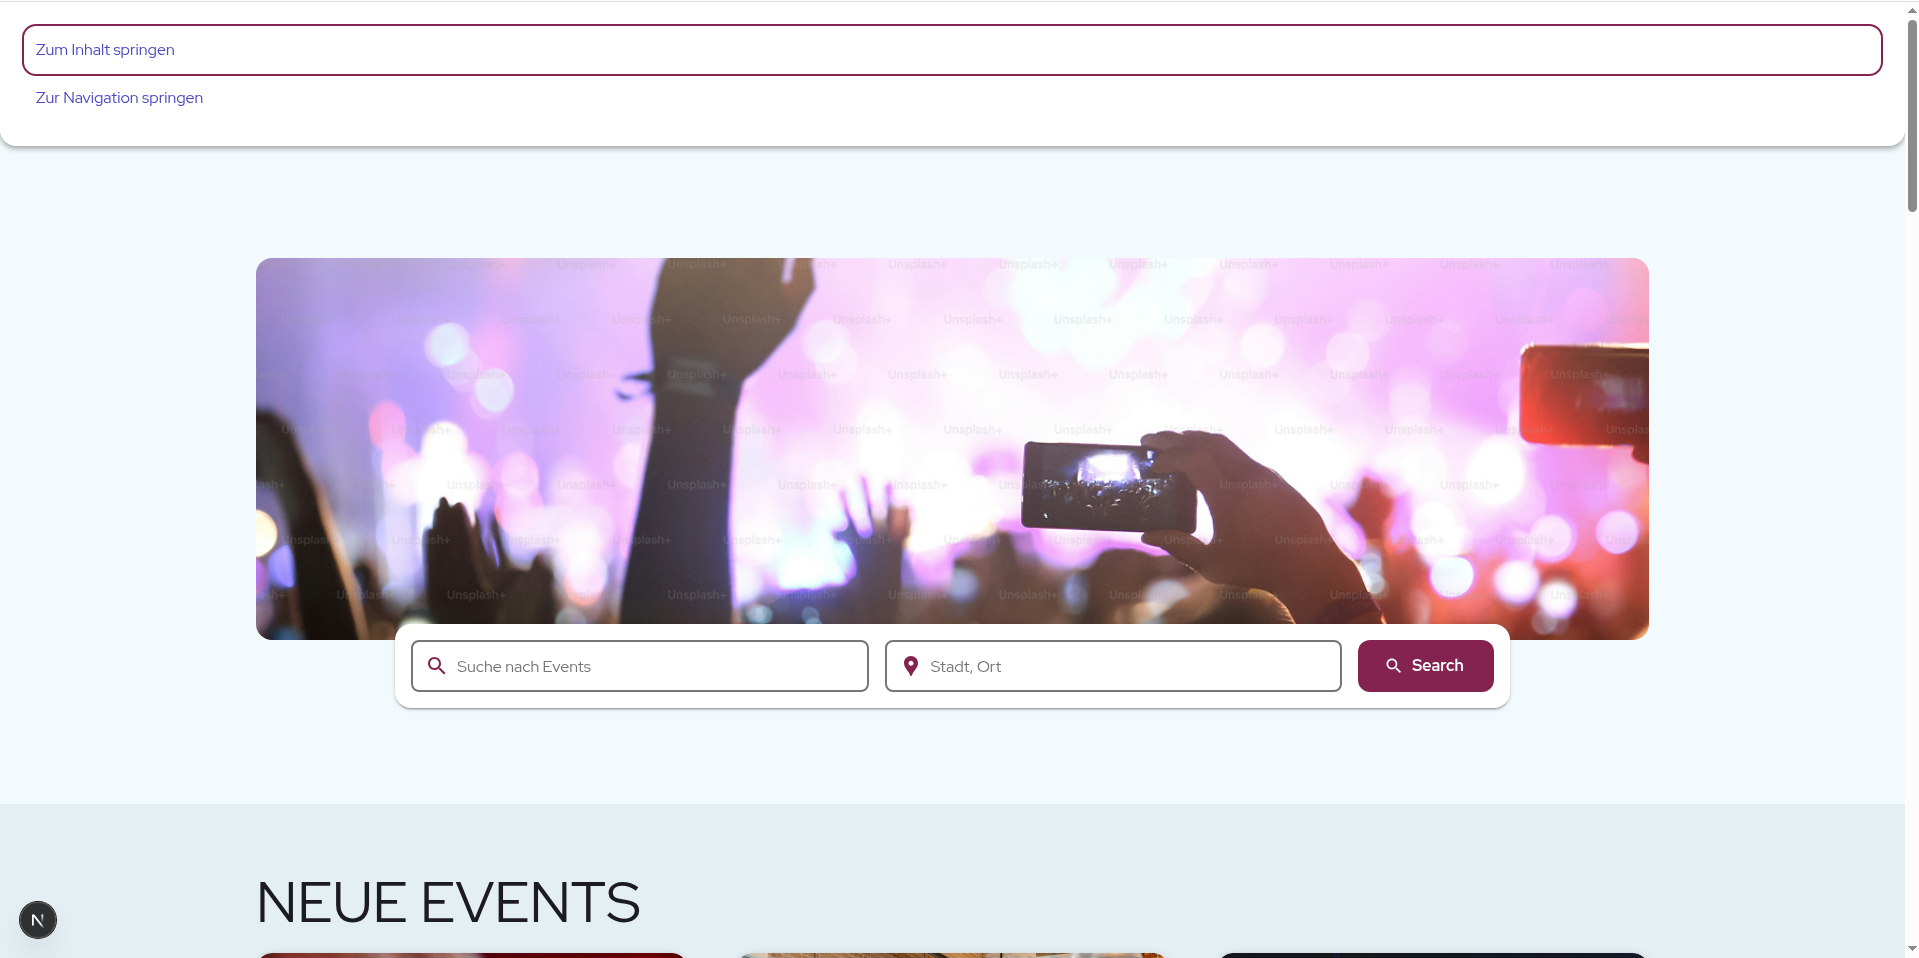
\includegraphics[width=\textwidth]{img/eventa11y_skip-links.png}
    \caption{Skip Links zum Überspringen der Navigation}
\end{figure}

Grundlegend aber trotzdem wichtig: Auch das Attribut \codeinline{lang=de} wurde angegeben, damit die Sprache definiert ist (3.1.1 Language of Page). Da die gesamte Website auf Deutsch ist fällt das Kriterium 3.1.2 Language of Parts weg.

\section{Navigationskonzept und Header}

Um eine konsistente Navigation zu bieten, wurde die Komponente der Navigation im Base-Layout fest integriert. So ist diese auf jeder Seite gleich strukturiert und erfüllt 3.2.3 Consistent Navigation. Die Navigation ist einer der aufwendigsten Komponenten, da es eine deutlich andere Darstellung im mobilen, als im Desktop erfordert. So werden die Menüpunkte nicht mehr angezeigt auf mobil, sondern können über einen Toggle Button sichtbar gemacht werden. Hierbei wurde darauf geachtet, dass das Menü auf wirklich ausgeblendet ist mit \codeinline{display: none}, sodass es auch im DOM nicht erscheint. Der Vorteil dabei ist, dass es dadurch nicht im Fokus Fluss aufrufbar ist, solange man es nicht über den Toggle Button einblendet. So muss man z.B. mit der Tastatur nicht durch jeden Menüpunkt einzeln navigieren um an sein Zeil zu gelangen. 

Da es sich bei dem Toggle Button um einen Button handelt, der das Menü auf- und zuklappt, wurden auch ARIA-Attribute verwendet um den aktuellen State anzuzeigen. Im initialen State wird der Button mit ARIA \codeinline{aria-label="Menü öffnen"} und \codeinline{aria-expanded="false"} beschrieben. Sobald man mit dem Button das Menü aktiviert ändern sich diese Attribute auf \codeinline{aria-label="Menü schließen"} und \codeinline{aria-expanded="true"}. Dies ist auch ein gutes Beispiel dafür, dass ARIA wirklich nur als Erweiterung von HTML gesehen werden sollte. Alles was das HTML nativ zur Verfügung stellt, sollte auch genutzt werden. Darüber hinaus, wie State Änderungen im Menü, müssen dann mit ARIA umgesetzt werden um Usern, die darauf angewiesen sind, diese Informationen mitzuteilen zu können.

\section{Formulare und Fehlermeldungen}

Genau wie bei der Navigation, sollte man einen besonderen Fokus auf Formulare legen. Formulare beinhalten Elemente die Interaktion erfordern. Dabei muss auch ausreichendes Feedback für den User bereitgestellt werden.

In dieser Anwendung wurde mithilfe von react-hook-form und der Validierungsbibliothek \codeinline{zod} das Daten und Fehlerhandling der einzelnen Inputfelder umgesetzt. Zuallerst wurde jedem Input auch ein Label zugewiesen, damit der User auch erkennt, welche Input Daten erwartet werden.

Auch die Suche ist ein Formular, welches eine Besonderheit bei den Labels aufweist. Diese wurden hier nämlich ausgeblendet um redundante Informationen für Sehende Personen zu verhindern. In diesem Fall benötigt man keine sichtbaren Labels \parencite[vgl.][]{w3c_hiding-labels_2025}. Zusätzlich wird neben den Ergebnissen auch eine Zusammenfassung angezeigt, die aussagt, wieviele Ergebnisse gefunden wurden (\href{https://www.w3.org/TR/WCAG21/#status-messages}{4.1.3 Status Messages})

Sollte eine fehlerhafte oder gar keine Eingabe erfolgt sein, die aber als erforderlich gekennzeichnet war, muss dem Benutzer klar der entsprechende Fehlerzustand angezeigt werden. Dabei wird sich nicht nur auf die Farbe verlassen (\href{https://www.w3.org/TR/WCAG21/#use-of-color}{1.4.1 Use of Color}), sondern erfolgt dann in Form eines Helfer Textes unter dem Input Feld, der genau beschreibt, was der Fehler ist. Der Vergleich zwischen der farbigen und der schwarz-weißen Ansicht zeigt auf warum Helfer Texte unter Input Feldern so wichtig sind. Nutzt man nur die Farbe um auf Fehler hinzuweisen, ist nicht erkenntlich wo der Fehler liegt. Zumal auch eine nicht farbenblinde Person nicht verstehen würde worin genau der Fehler liegt, ohne vernünftige Beschreibung.

\begin{figure}[H]
    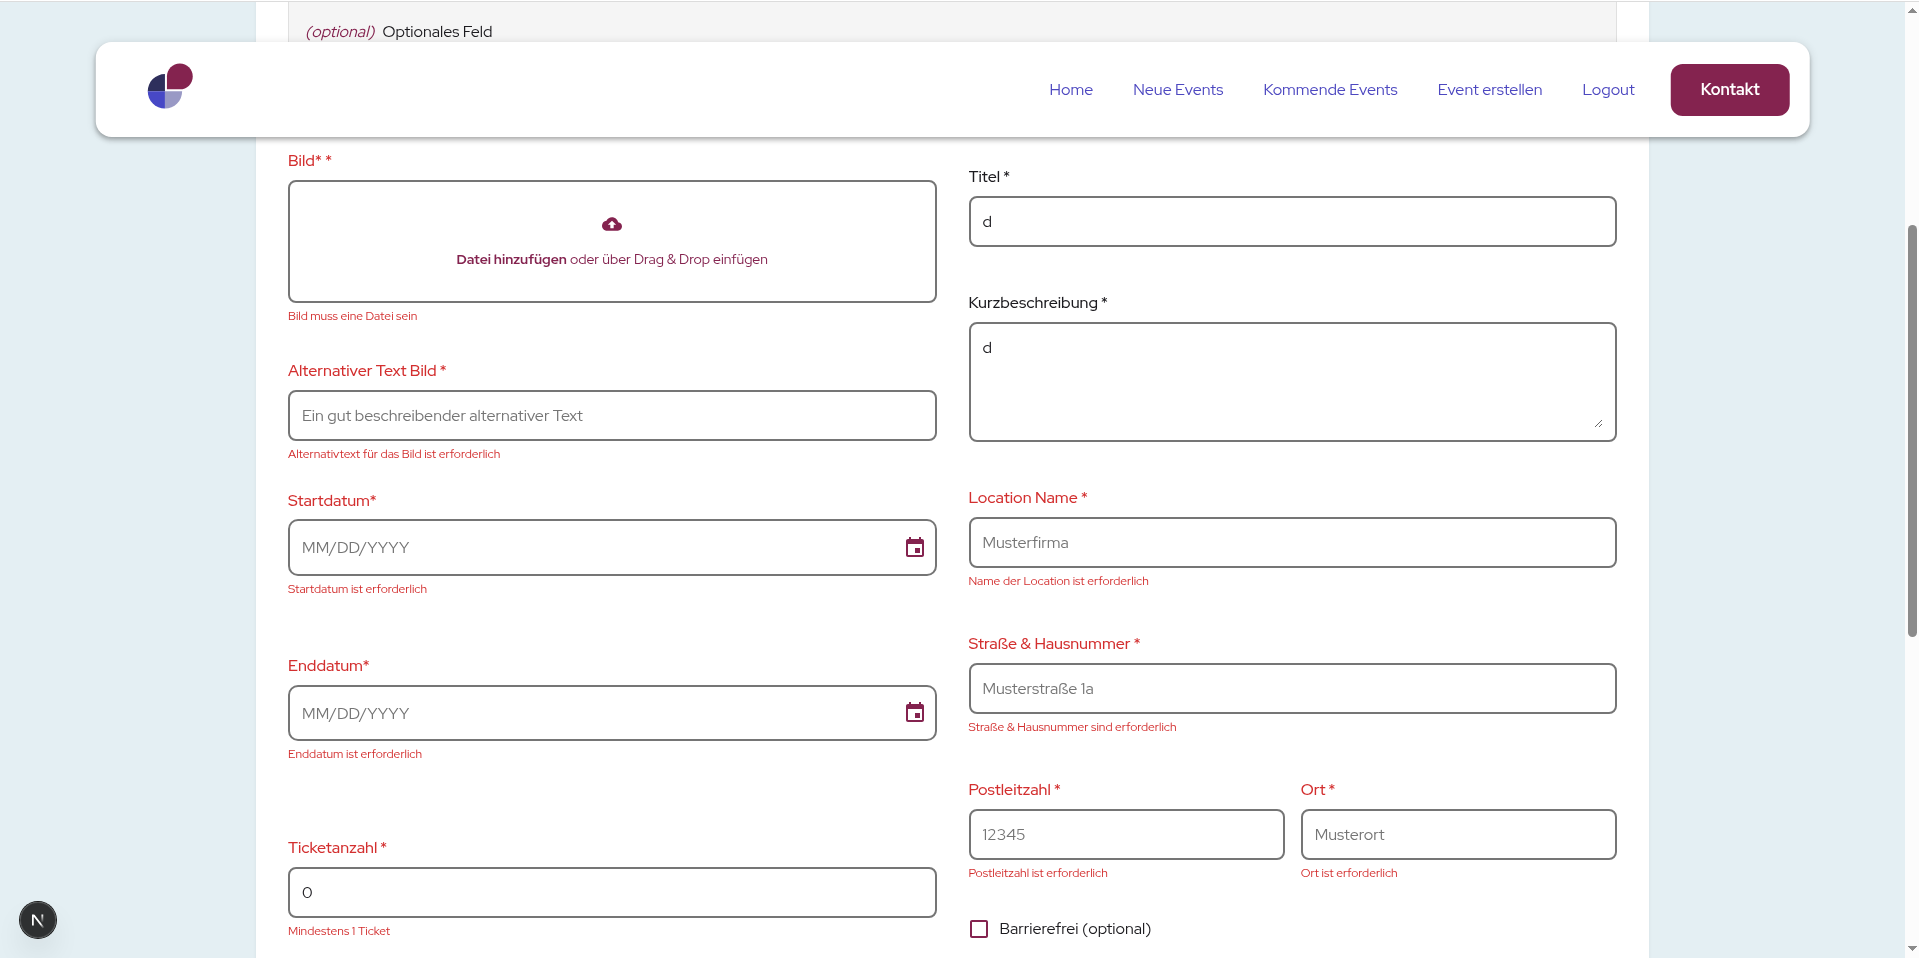
\includegraphics[width=\textwidth]{img/eventa11y_helpertext.png}
    \caption{Form Errors mit Helfer Texten in Farbe}
\end{figure}

\begin{figure}[H]
    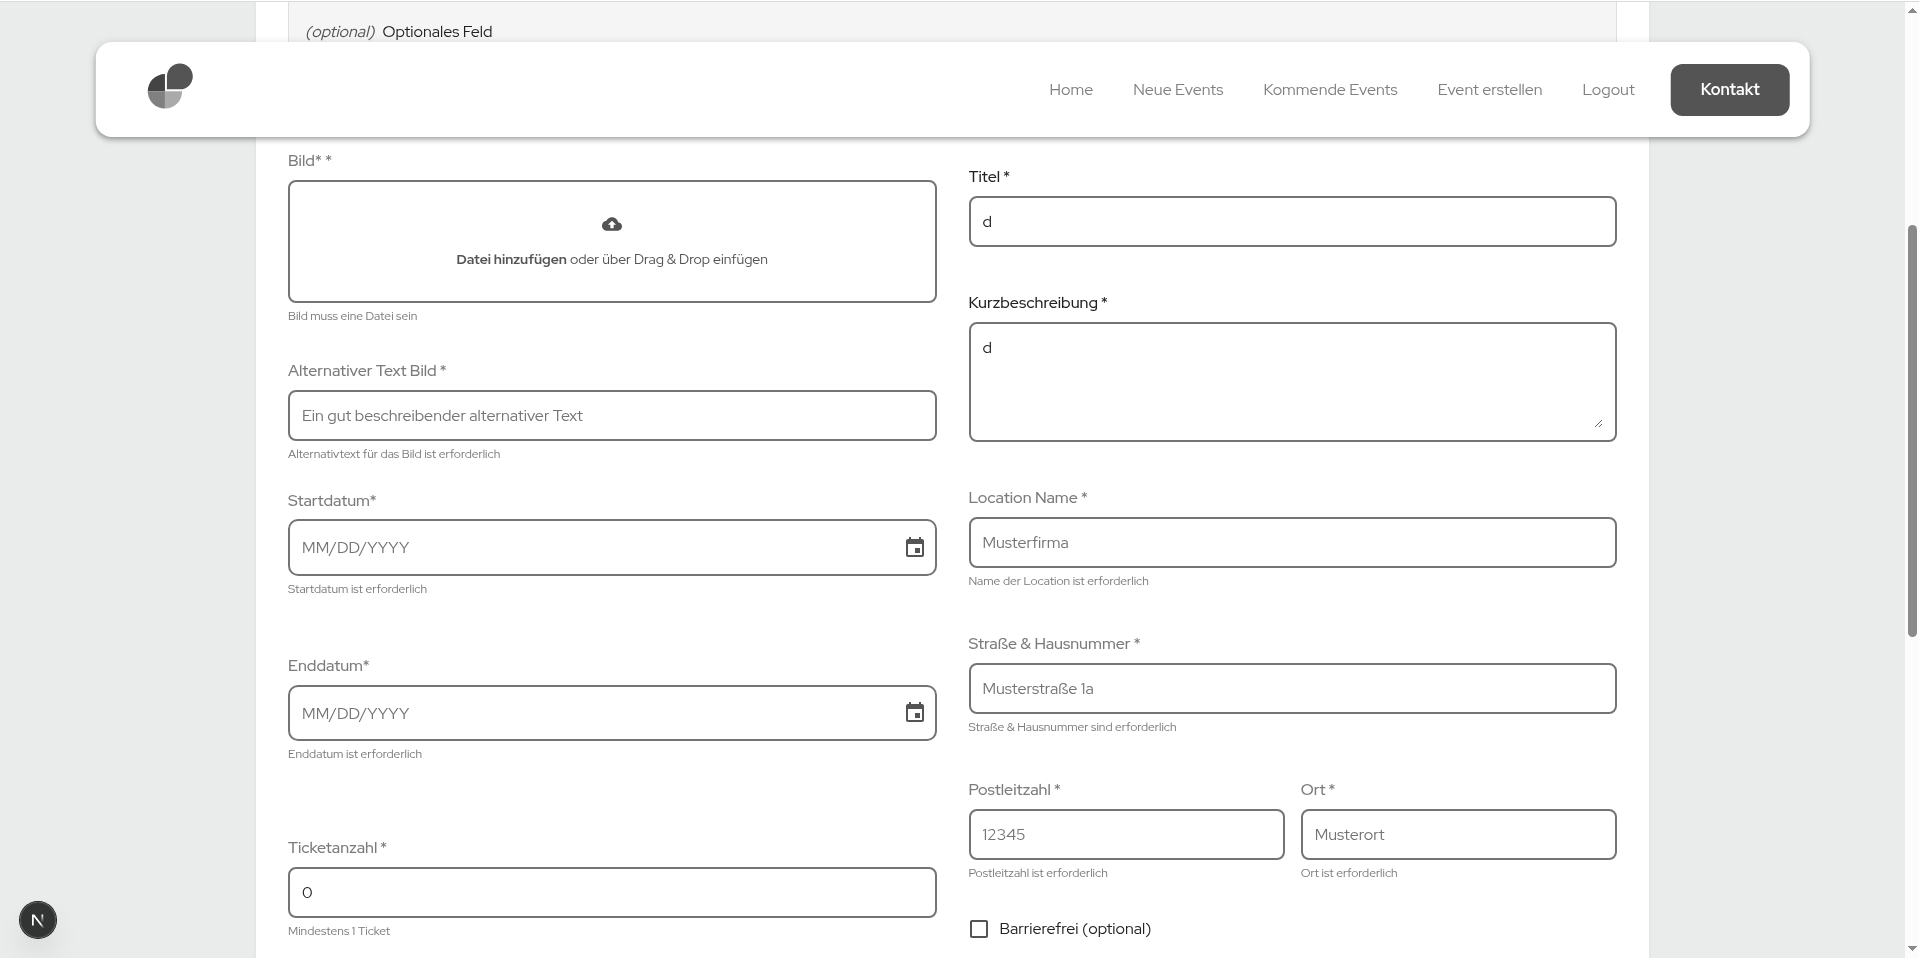
\includegraphics[width=\textwidth]{img/eventa11y_helpertext_grey.png}
    \caption{Form Errors mit Helfer Texten in schwarz-weiß}
\end{figure}

Zusätzlich wird das Input Feld auch wieder mit ARIA beschrieben. \codeinline{aria-invalid="true"} zeigt dem User, ob die Input Eingabe valide ist oder nicht. 

Im Kontaktformular wurde auch das Input Attribut \codeinline{autocomplete} verwendet. Damit kann angegeben werden ob und welche Berechtigung der User-Agent (z.B. der Browser) hat, automatische Hilfe beim Ausfüllen von Formularfeldern zu leisten. Auch wird beschrieben, welche Art von Information von dem Feld erwartet werden. Dafür wird aus einem festgelegtem Set an Optionen ausgewählt.

\begin{figure}[H]
\begin{minted}[linenos, bgcolor=gray!10]{tsx}
<InputField
  name="lastName"
  label="Nachname*"
  register={register}
  error={errors.lastName?.message}
  placeholder="Mustermann"
  autocomplete="family-name"
/>
\end{minted}
\caption{Ein Input Field als React Komponente mit \codeinline{autocomplete} und Errors mit zod und react-hook-form}
\end{figure}

\section{Statusmeldungen und Snackbar-Komponenten}
Benutzer werden bei Statusmeldungen, wie etwas beim Absenden eines Formulars, visuell und auditiv informiert. Die Snackbar-Komponente von notistack verwendet die \codeinline{role="alert"}. Zusätlich wurde individuell ein Schließen Button eingefügt. Dadurch wird zum einen gewährleistet, dass Screenreader die Statusmeldung gleich vorliest \parencite[vgl.][]{mdn_role-alert_nodate}, wenn sie erscheint und zum anderen der User die Möglichkeit hat die Statusmeldung auch wegzuklicken. Letzteres gibt Kriterium \href{https://www.w3.org/TR/WCAG21/#timing-adjustable}{2.2.1 Timing Adjustable Turn off} vor.

Die Snackbar von notistack war allerdings noch nicht barrrierefrei und musste noch einmal, in der Schriftgröße und Schriftdicke angepasst werden um dem Kriterium \href{https://www.w3.org/TR/WCAG21/#contrast-minimum}{1.4.3 Contrast (Minimum)} gerecht zu werden.

\section{Responsivität und Reflow}
Die Anwendung passt sich unterschiedlichen Bildschirmgrößen an. Karten-Layouts etwa brechen von einer Drei-Spalten-Ansicht auf eine Ein-Spalten-Ansicht herunter (\href{https://www.w3.org/TR/WCAG21/#reflow}{1.4.10 Reflow}). Damit wird auch das Kriterium \href{https://www.w3.org/TR/WCAG21/#orientation}{1.3.4 Orientation erfüllt}.

\section{Fehlervermeidung und Bestätigung}
Vor dem finalen Absenden eines Buchungsprozesses gibt es eine Übersichtsseite, um Eingaben zu überprüfen. Dies unterstützt \href{https://www.w3.org/TR/WCAG21/#error-prevention-legal-financial-data}{3.3.4 Error Prevention (Legal, Financial, Data)}. Kontextänderungen durch Fokus oder Eingabe wurden bewusst vermieden (\href{https://www.w3.org/TR/WCAG21/#on-focus}{3.2.1 On Focus}, \href{https://www.w3.org/TR/WCAG21/#on-input}{3.2.2 On Input}). Das heißt, dass sich die Seite um das Feld sich nicht insoweit verändert, dass der Kontext nicht mehr verstanden wird.

\section{Hinweise zu nicht implementierten Bereichen}
Da es keine Videoinhalte auf der Eventplatform gibt, konnten die dazu gehörigen Kriterien, wie zum Beispiel 2.2.2 Pause, Stop, Hide (z. B. für Multimedia-Inhalte) oder 1.2.2 Captions (Prerecorded) auch nicht umgesetzt werden. 

\section{Ausblick: Progressive Enhancement}
Ein sinnvoller Ausblick für zukünftige Entwicklungen liegt in der Progressive Enhancement-Strategie: Inhalte sollten auch ohne JavaScript zugänglich sein. Die derzeitige Anwendung setzt noch stark auf clientseitiges Rendering und ist ohne JavaScript nur begrenzt benutzbar.
